\section{Anisotropia de forma}

Conforme dito na seção 4.2 existe uma relação entre os elementos do tensor de depolarização e os semi-eixos. Na Figura \ref{fig:ellipsoid_shape_iso10} mostramos como o aumento do semi-eixo maior afeta o vetor de magnetização resultante. A princípio, os três semi-eixos estão muito próximos, simulando uma esfera. Quando postos sob um campo externo, o vetor de magnetização resultante se direciona para a direção deste campo. Porém a medida que aumenta-se o semi-eixo maior, ocorre a depolarização dos demais e o vetor de magnetização resultante tende a se alinhar na direção do semi-eixo maior (neste caso o elipsoide triaxial possui um azimute de 10$º$).

\vspace{2cm}

\begin{table}[h!]
	\begin{center}
		\begin{tabular}{|l|c|c|}
			\hline
			\textbf{Parâmetro}  & \textbf{Valor}  & \textbf{Unidade }\\
			\hline 
			a, b, c  & 50.1-1000, 50, 49.9 & m\\
			\hline
			Azimute   & $10$ & º \\
			\hline
			$\delta$    & $0$ & º\\
			\hline
			$\gamma$   & $0$  & º\\
			\hline
			xc   & 0  & m\\
			\hline          
			yc   & 0  & m\\
			\hline                
			zc   & 1000  & m\\
			\hline
			$J_{NRM}$*  & 100, $0^o$, $0^o$ & A/m \\
			\hline
			F*    & 60000, $90^o$, $20^o$ & nT\\
			\hline
			k1, k2, k3   & 50, 50, 50  & SI\\
			\hline
			Orientações k**   & $0$, $90$, $90$  & º\\
			\hline
		\end{tabular}
		\caption{Parâmetros do elipsoide triaxial modelado. *Valores de intensidade, inclinação e declinação respectivamente. **Ângulo de \textit{strike} , \textit{dip}  e \textit{rake} , respectivamente, para calcular os vetores unitários $\mathbf{u}_{1}$, $\mathbf{u}_{2}$, $\mathbf{u}_{3}$ por meio das Eqs. \ref{eq:v1_triaxial_prolate}, \ref{eq:v2_triaxial_prolate} e \ref{eq:v3_triaxial_prolate}.}
	\end{center}
	\label{tab:ellipsoid_shape_iso10}
\end{table}

\begin{table}[h!]
	\begin{center}
		\begin{tabular}{lc}
			
			&  \\
			& \\
			& \\
			&  \\
			& \\
			& \\
			& \\
			& \\
			& \\
			& \\
			
			
		\end{tabular}
	\end{center}
\end{table}

\begin{figure}[hbt!]
	\centering 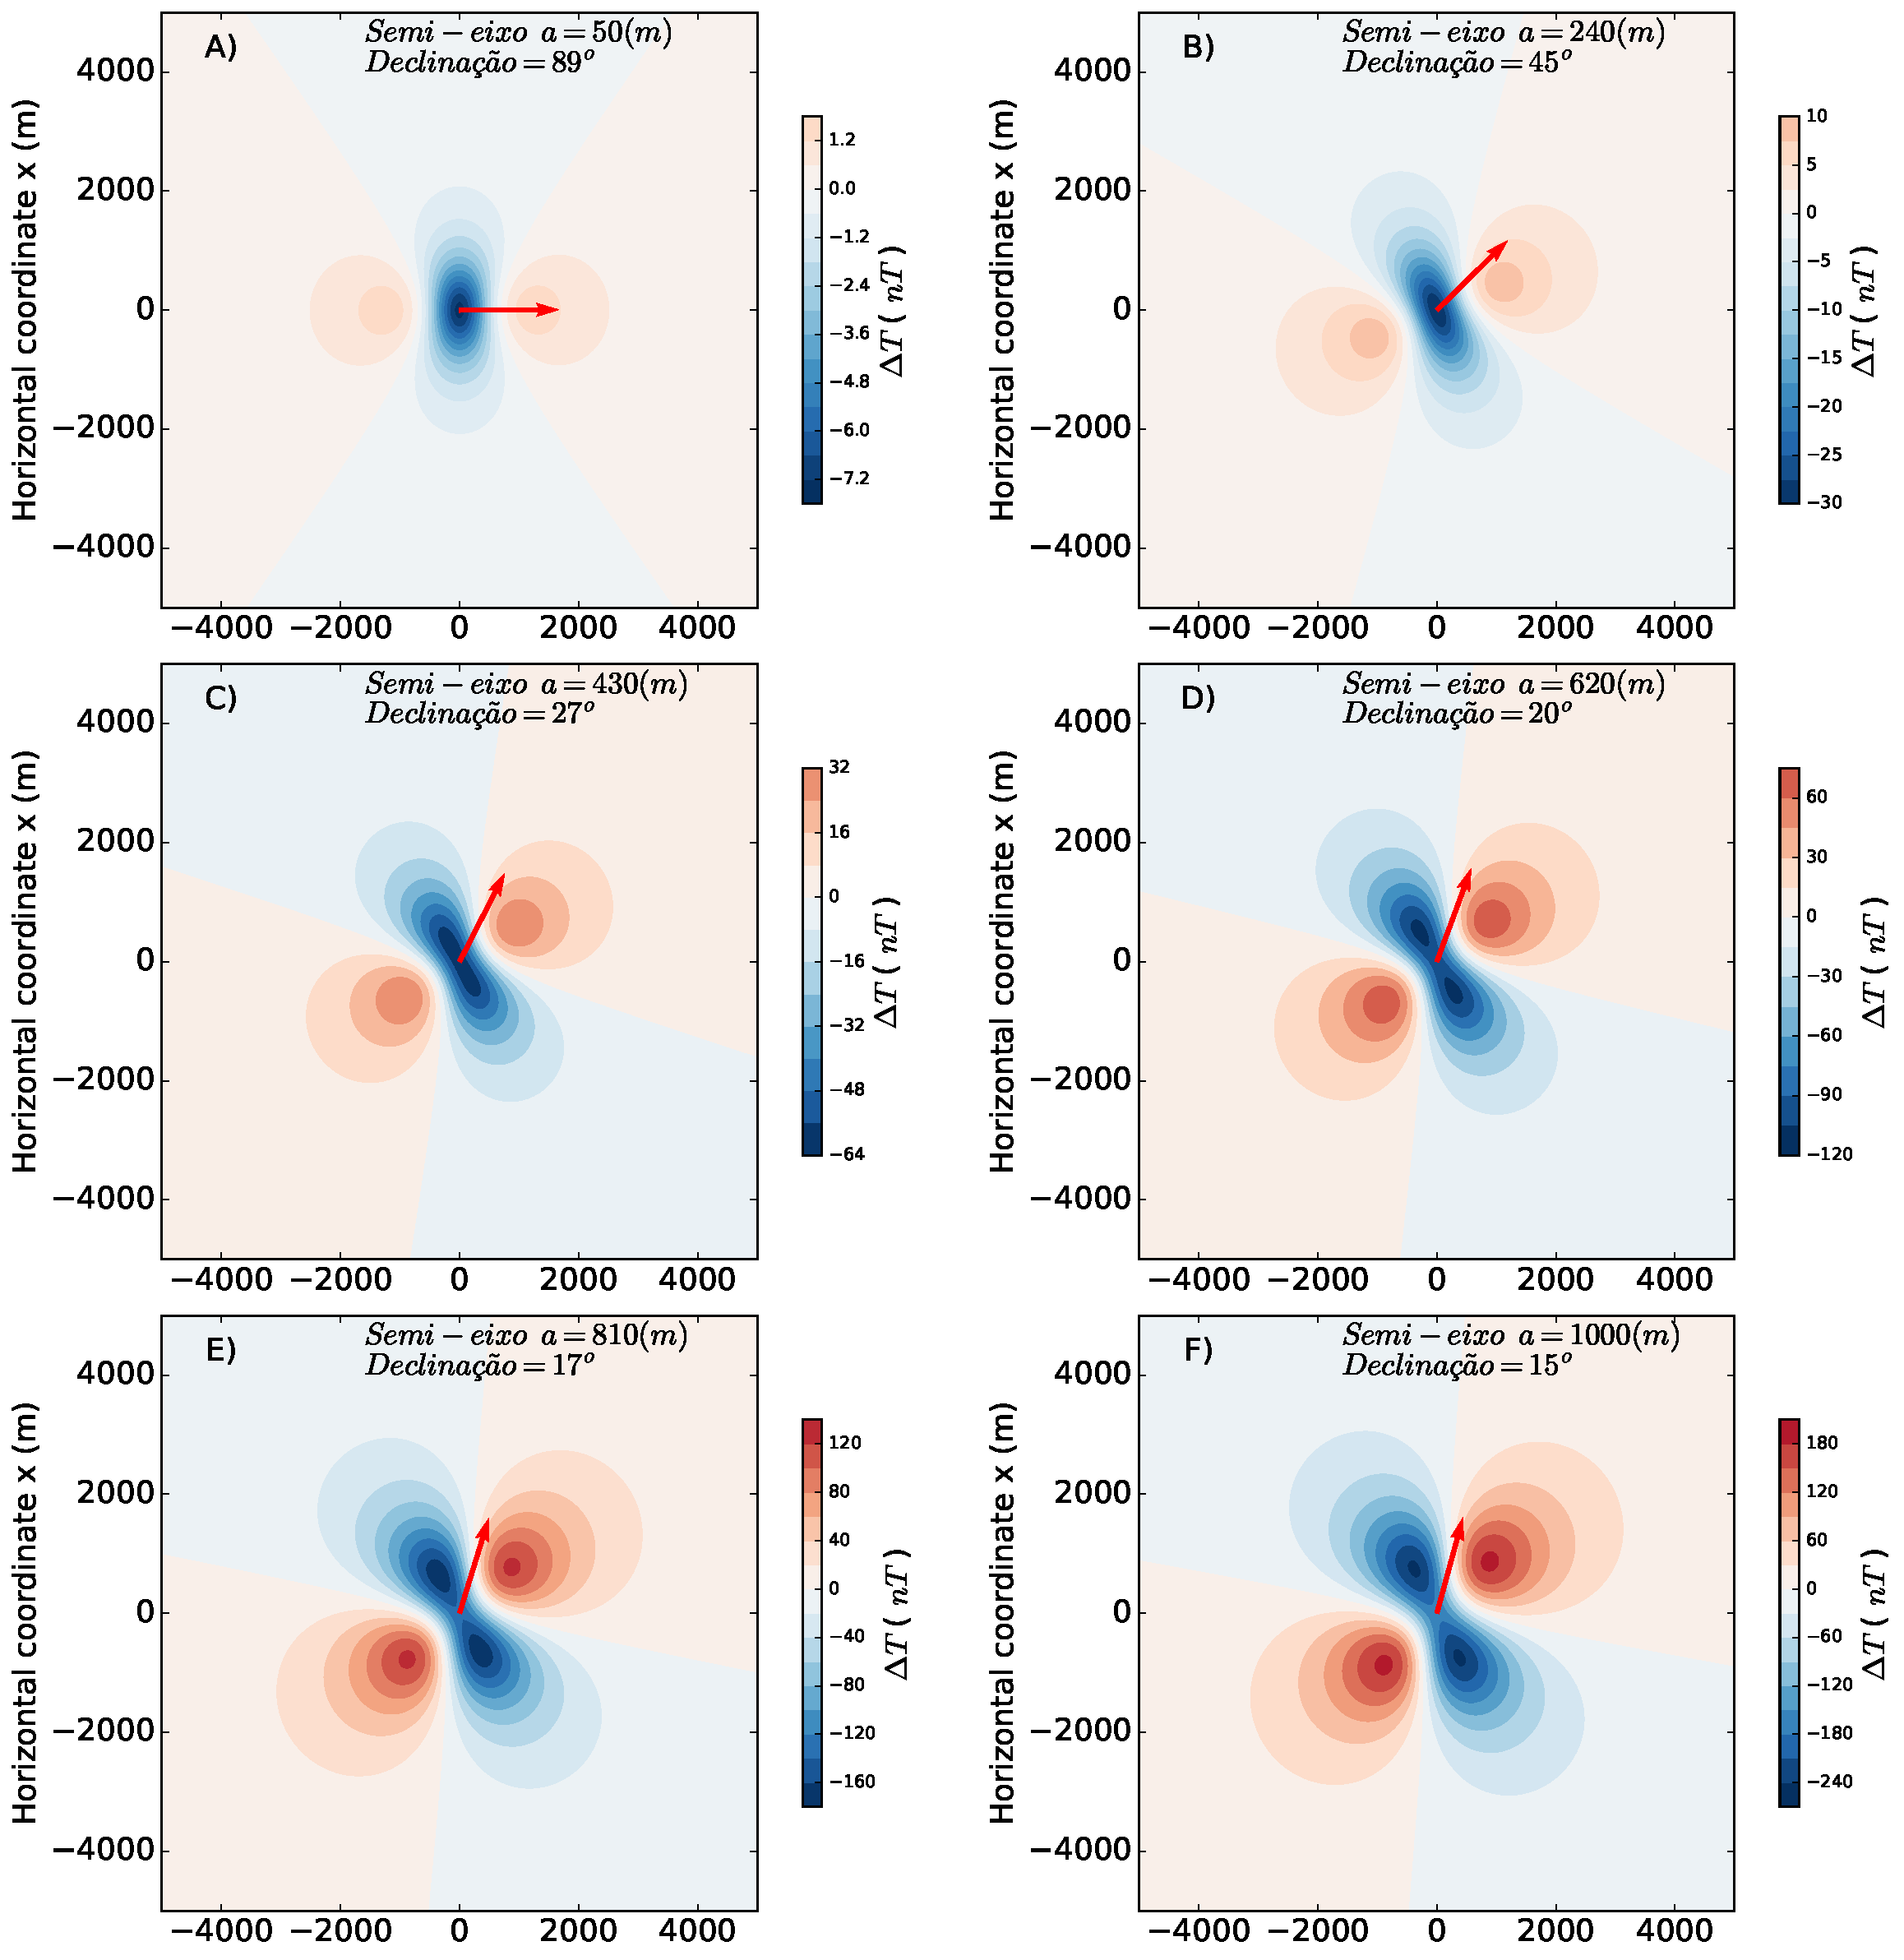
\includegraphics[width=16 cm,height=16 cm]{figures/ellipsoid_shape_iso}
	\caption[Simulação, da mudança do vetor de magnetização resultante, de um elipsoide triaxial com o aumento do semi-eixo maior.]{Simulação, da mudança do vetor de magnetização resultante, de um elipsoide triaxial com o aumento do semi-eixo maior. O elipsoide está imerso em um campo externo constante de declinação $90^o$, possui susceptibilidade isotrópica e constante e está direcionado com um azimute de $10^o$. Ao longo da sequência das figuras, seu semi-eixo maior aumenta de proporção em relação aos demais (variando entre 50 e 3000 m.). Nota-se a tendência do vetor de magnetização resultante (seta em vermelho) em se alinhar com o semi-eixo maior.}
	\label{fig:ellipsoid_shape_iso10}
\end{figure}

\begin{table}[h!]
	\begin{center}
		\begin{tabular}{lc}
			
			& \\
			& \\
			& \\
			& \\
			& \\
			
		\end{tabular}
	\end{center}
\end{table}

Para efeito de comparação realizamos o mesmo teste, porém com um azimute de 80$º$ para o elipsoide. A variação é bem menor, mas também se confirma a tendência do alinhamento do vetor de magnetização resultante para a direção do semi-eixo maior.

\vspace{2cm}

\begin{table}[h!]
	\begin{center}
		\begin{tabular}{|l|c|c|}
			\hline
			\textbf{Parâmetro}  & \textbf{Valor}  & \textbf{Unidade} \\
			\hline 
			a, b, c & 50.1-1000, 50, 49.9 & m\\
			\hline
			Azimute   & $80$ & º\\
			\hline
			$\delta$    & $0$ & º\\
			\hline
			$\gamma$   & $0$  & º\\
			\hline
			xc   & 0  & m\\
			\hline          
			yc   & 0  & m\\
			\hline                
			zc   & 1000  & m\\
			\hline
			$J_{NRM}$*  & 100, $0^o$, $0^o$  & A/m\\
			\hline
			F*    & 60000, $50^o$, $20^o$ & nT\\
			\hline
			k1, k2, k3   & 50, 50, 50  & SI\\
			\hline
			Orientações k**   & $0$, $90$, $90$  & º\\
			\hline
		\end{tabular}
		\caption{Parâmetros do elipsoide triaxial modelado. *Valores de intensidade, inclinação e declinação respectivamente. **Ângulo de \textit{strike} , \textit{dip}  e \textit{rake} , respectivamente, para calcular os vetores unitários $\mathbf{u}_{1}$, $\mathbf{u}_{2}$, $\mathbf{u}_{3}$ por meio das Eqs. \ref{eq:v1_triaxial_prolate}, \ref{eq:v2_triaxial_prolate} e \ref{eq:v3_triaxial_prolate}.}
	\end{center}
	\label{tab:ellipsoid_shape_iso80}
\end{table}

\begin{figure}[hbt!]
	\centering 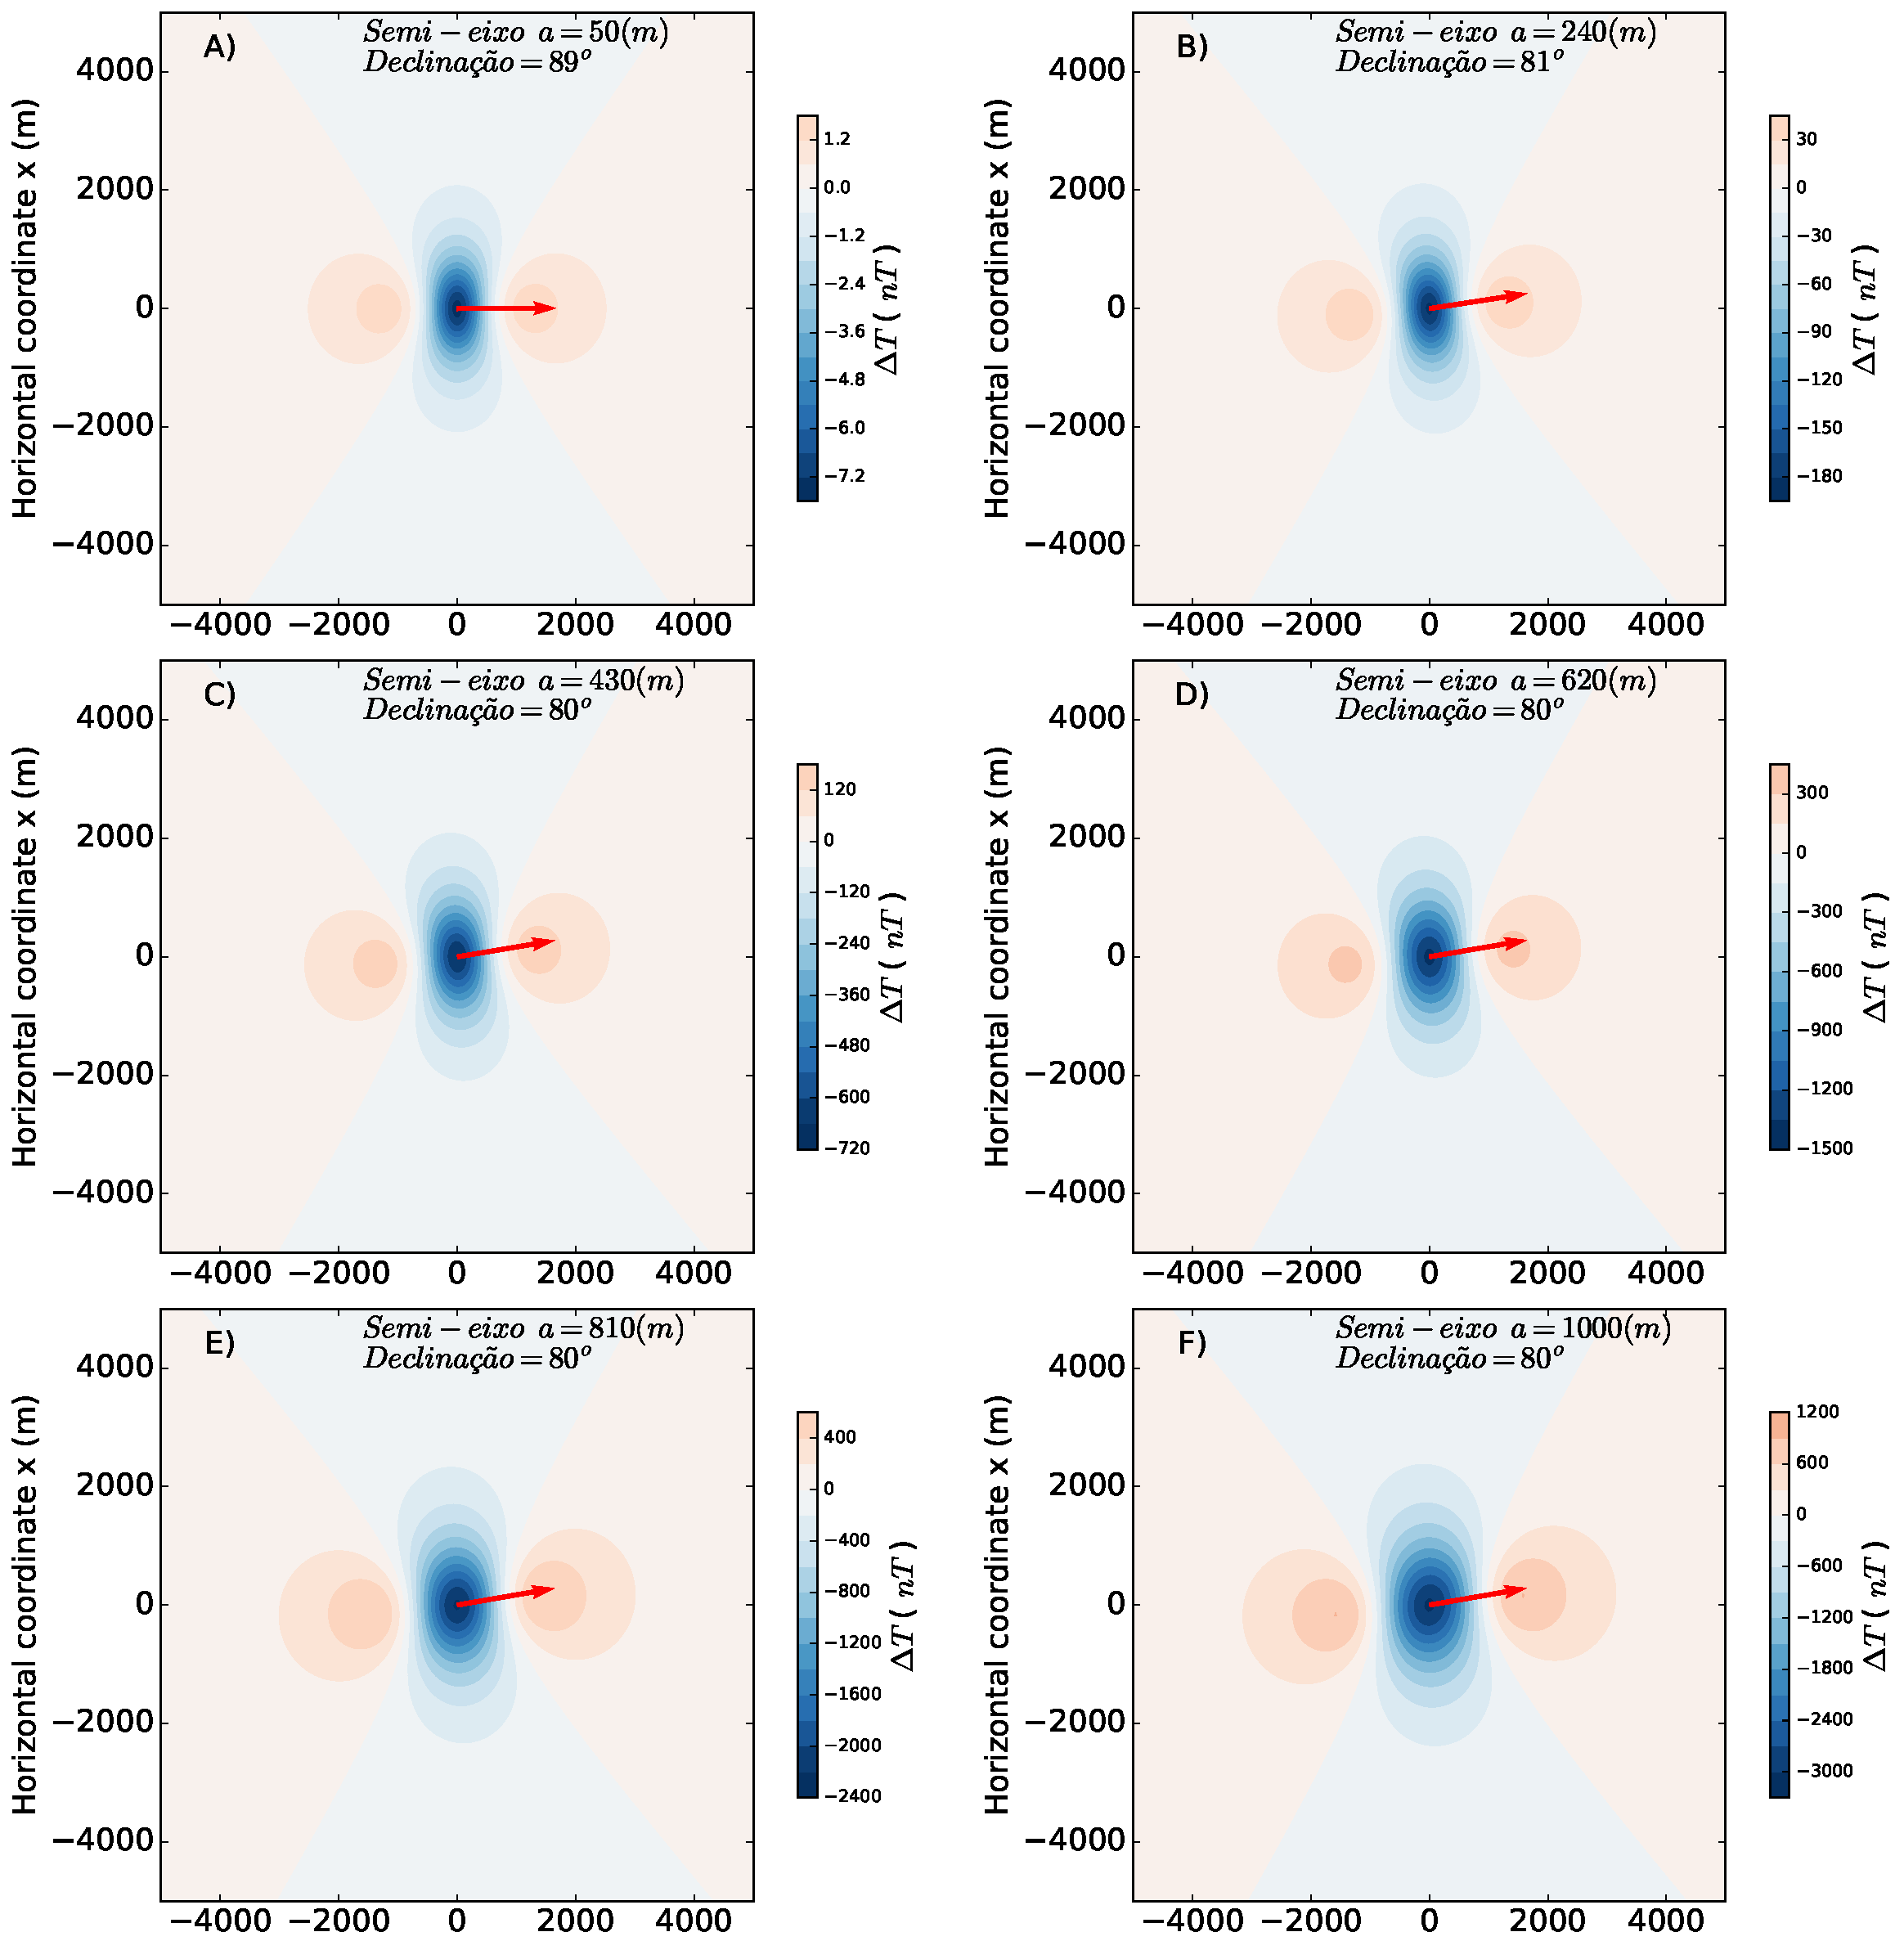
\includegraphics[width=16 cm,height=16 cm]{figures/ellipsoid_shape_iso2}
	\caption[Simulação, da mudança do vetor de magnetização resultante, de um elipsoide triaxial com o aumento do semi-eixo maior.]{Simulação, da mudança do vetor de magnetização resultante, de um elipsoide triaxial com o aumento do semi-eixo maior. O elipsoide está imerso em um campo externo constante de declinação $90^o$, possui susceptibilidade constante e direcionado com um azimute de $80^o$. Ao longo da sequência das figuras, seu semi-eixo maior aumenta de proporção em relação aos demais (variando entre 50 e 3000 m.). Nota-se a tendência do vetor de magnetização resultante (seta em vermelho) em se alinhar com o semi-eixo maior. Diferente da figura anterior, houve pouca mudança na declinação devido ao alinhamento do elipsoide com a campo externo.}
	\label{fig:ellipsoid_shape_iso80}
\end{figure}


Em outro teste que foi conduzido, verificamos a mudança de direção do vetor de magnetização, com a tendência de se alinhar ao semi-eixo maior do elipsoide conforme este aumentava, mesmo com uma susceptibilidade ($k_1$, $k_2$ e $k_3$) constante. Isto, se deve ao fato que o semi-eixo maior sofrerá menor desmagnetização que os demais, o que é chamado de anisotropia de susceptibilidade de forma.